%%% Verze pro jednostranný tisk:
\documentclass[11pt,a4paper]{report}
\usepackage[top=25mm,bottom=25mm,right=25mm,left=30mm,head=12.5mm,foot=12.5mm]{geometry}
\let\openright=\clearpage

%%% Pokud tiskneme oboustranně:
%\documentclass[11pt,a4paper,twoside,openright]{report}
%\usepackage[top=25mm,bottom=25mm,right=25mm,left=30mm,head=12.5mm,foot=12.5mm]{geometry}
%\let\openright=\cleardoublepage

%%% Definice různých užitečných maker (viz popis uvnitř souboru)
%%% Tento soubor obsahuje definice různých užitečných maker a prostředí %%%
%%% Další makra připisujte sem, ať nepřekáží v ostatních souborech.     %%%
%%% This file contains definitions of various useful macros and environments      %%%
%%% Assign additional macros here so that they do not interfere with other files. %%%

\usepackage[a-2u]{pdfx}     % výsledné PDF bude ve standardu PDF/A-2u
                            % resulting PDF will be in the PDF / A-2u standard

\usepackage{ifpdf}
\usepackage{ifxetex}
\usepackage{ifluatex}

%%% Nastavení pro použití samostatné bibliografické databáze.
%%% Settings for using a separate bibliographic database.
\usepackage[
   backend=biber
%  ,style=iso-authoryear
  ,style=iso-numeric
  ,sortlocale=cs_CZ
  ,alldates=iso
  ,bibencoding=UTF8
  ,maxnames=2
  ,maxbibnames=99
  %,block=ragged
]{biblatex}
\let\cite\parencite
\renewcommand*{\multinamedelim}{, \addspace}
\renewcommand*{\finalnamedelim}{\addspace a \addspace}

\bibliography{literatura}

%% Přepneme na českou sazbu, fonty Latin Modern a kódování češtiny
\ifthenelse{\boolean{xetex}\OR\boolean{luatex}}
   { % use fontspec and OpenType fonts with utf8 engines
			\usepackage[english,slovak,czech]{babel}
			\usepackage[autostyle,english=british,czech=quotes]{csquotes}
			\usepackage{fontspec}
			\defaultfontfeatures{Ligatures=TeX,Scale=MatchLowercase}
   }
   {
			\usepackage[english,slovak,czech]{babel}
			\usepackage{lmodern}
			\usepackage[T1]{fontenc}
			\usepackage{textcomp}
			\usepackage[utf8]{inputenc}
			\usepackage[autostyle,english=british,czech=quotes]{csquotes}
	 }
\ifluatex
\makeatletter
\let\pdfstrcmp\pdf@strcmp
\makeatother
\fi

%%% Další užitečné balíčky (jsou součástí běžných distribucí LaTeXu)
\usepackage{amsmath}        % rozšíření pro sazbu matematiky / extension for math typesetting
\usepackage{amsfonts}       % matematické fonty / mathematical fonts
\usepackage{amssymb}        % symboly / symbols
\usepackage{amsthm}         % sazba vět, definic apod. / typesetting of sentences, definitions, etc.
\usepackage{bm}             % tučné symboly (příkaz \bm) / bold symbols (\bm command)
\usepackage{graphicx}       % vkládání obrázků / graphics inserting
\usepackage{listings}       % vylepšené prostředí pro strojové písmo / improved environment for source codes typesetting
\usepackage{fancyhdr}       % prostředí pohodlnější nastavení hlavy a paty stránek / environment for more comfortable adjustment of the head and foot of the pages
\usepackage{icomma}         % inteligetní čárka v matematickém módu / intelligent comma in math mode
\usepackage{dcolumn}        % lepší zarovnání sloupců v tabulkách / better alignment of columns in tables
\usepackage{booktabs}       % lepší vodorovné linky v tabulkách / better horizontal lines in tables
\makeatletter
\@ifpackageloaded{xcolor}{
   \@ifpackagewith{xcolor}{usenames}{}{\PassOptionsToPackage{usenames}{xcolor}}
  }{\usepackage[usenames]{xcolor}} % barevná sazba / color typesetting
\makeatother
\usepackage{multicol}       % práce s více sloupci na stránce / work with multiple columns on a page
\usepackage{caption}
\usepackage{enumitem}
\setlist[itemize]{noitemsep, topsep=0pt, partopsep=0pt}
\setlist[enumerate]{noitemsep, topsep=0pt, partopsep=0pt}
\setlist[description]{noitemsep, topsep=0pt, partopsep=0pt}

\usepackage{tocloft}
\setlength\cftparskip{0pt}
\setlength\cftbeforechapskip{1.5ex}
\setlength\cftfigindent{0pt}
\setlength\cfttabindent{0pt}
\setlength\cftbeforeloftitleskip{0pt}
\setlength\cftbeforelottitleskip{0pt}
\setlength\cftbeforetoctitleskip{0pt}
\renewcommand{\cftlottitlefont}{\Huge\bfseries\sffamily}
\renewcommand{\cftloftitlefont}{\Huge\bfseries\sffamily}
\renewcommand{\cfttoctitlefont}{\Huge\bfseries\sffamily}

% vyznaceni odstavcu
% differentiation of new paragraphs
\parindent=0pt
\parskip=11pt

% zakaz vdov a sirotku - jednoradkovych pocatku ci koncu odstavcu na prechodu mezi strankami
% Prohibition of widows and orphans - single-line beginning and end of paragraph at the transition between pages
\clubpenalty=1000
\widowpenalty=1000
\displaywidowpenalty=1000

% nastaveni radkovani
% setting of line spacing
\renewcommand{\baselinestretch}{1.20}

% nastaveni pro nadpisy - tucne a bezpatkove
% settings for headings - bold and sans serif
\usepackage{sectsty}    
\allsectionsfont{\sffamily}

% nastavení hlavy a paty stránek
% page head and foot settings
\makeatletter
\if@twoside%
    \fancypagestyle{fancyx}{%
			\fancyhf{}                                     
      \fancyhead[RE]{\rightmark}                  
      \fancyhead[LO]{\leftmark}                  
      \fancyfoot[RO,LE]{\thepage}                    
      \renewcommand{\headrulewidth}{.5pt}            
      \renewcommand{\footrulewidth}{.5pt}            
    }
    \fancypagestyle{plain}{%
			\fancyhf{}                                     
    	\fancyfoot[RO,LE]{\thepage}                    
    	\renewcommand{\headrulewidth}{0pt}             
    	\renewcommand{\footrulewidth}{0.5pt}
    }          
\else
    \fancypagestyle{fancyx}{%
			\fancyhf{}                                     
      \fancyhead[R]{\leftmark}                  
      \fancyfoot[R]{\thepage}                    
      \renewcommand{\headrulewidth}{.5pt}            
      \renewcommand{\footrulewidth}{.5pt}            
    }
    \fancypagestyle{plain}{%                       
    	\fancyhf{} % clear all header and footer fields
    	\fancyfoot[R]{\thepage}                    
    	\renewcommand{\headrulewidth}{0pt}             
    	\renewcommand{\footrulewidth}{0.5pt}
    }          
\fi
\renewcommand*{\cleardoublepage}{\clearpage\if@twoside \ifodd\c@page\else
	\hbox{}%
	\thispagestyle{empty}%
	\newpage%
	\if@twocolumn\hbox{}\newpage\fi\fi\fi
}
\makeatother

% Tato makra přesvědčují mírně ošklivým trikem LaTeX, aby hlavičky kapitol
% sázel příčetněji a nevynechával nad nimi spoustu místa. Směle ignorujte.
% These macros convince with a slightly ugly LaTeX trick to make chapter headers
% bet more sane and didn't miss a lot of space above them. Be boldly ignore it.
\makeatletter
\def\@makechapterhead#1{
  {\parindent \z@ \raggedright \sffamily
   \Huge\bfseries \thechapter. #1
   \par\nobreak
   \vskip 20\p@
}}
\def\@makeschapterhead#1{
  {\parindent \z@ \raggedright \sffamily
   \Huge\bfseries #1
   \par\nobreak
   \vskip 20\p@
}}
\makeatother

% Trochu volnější nastavení dělení slov, než je default.
% Slightly looser hyphenation setting than default.
\lefthyphenmin=2
\righthyphenmin=2

% Zapne černé "slimáky" na koncích řádků, které přetekly, abychom si jich lépe všimli.
% Turns on the black "snails" at the ends of the lines that overflowed to get us noticed them better.
\overfullrule=1mm

%% Balíček hyperref, kterým jdou vyrábět klikací odkazy v PDF,
%% ale hlavně ho používáme k uložení metadat do PDF (včetně obsahu).
%% Většinu nastavítek přednastaví balíček pdfx.
%% A hyperref package that can be used to produce clickable links in PDF,
%% but we mainly use it to store metadata in PDF (including content).
%% Most settings are preset by the pdfx package.
\hypersetup{unicode}
\hypersetup{breaklinks=true}
\hypersetup{hidelinks}

\renewcommand{\UrlBreaks}{\do\/\do\=\do\+\do\-\do\_\do\ \do\a\do\b\do\c\do\d%
\do\e\do\f\do\g\do\h\do\i\do\j\do\k\do\l\do\m\do\n\do\o\do\p\do\q\do\r\do\s%
\do\t\do\u\do\v\do\w\do\x\do\y\do\z\do\A\do\B\do\C\do\D\do\E\do\F\do\G\do\H%
\do\I\do\J\do\K\do\L\do\M\do\N\do\O\do\P\do\Q\do\R\do\S\do\T\do\U\do\V\do\W%
\do\X\do\Y\do\Z\do\1\do\2\do\3\do\4\do\5\do\6\do\7\do\8\do\9\do\0}

%%% Prostředí pro sazbu kódu, případně vstupu/výstupu počítačových
%%% programů. (Vyžaduje balíček listings -- fancy verbatim.)
%%% Environment for source code typesetting, or computer input/output
%%% programs. (Requires package listings - fancy verbatim.)
\lstnewenvironment{code}{\lstset{basicstyle=\small, frame=single}}{}



%%% DEFINICE ZÁKLADNÍCH PROMĚNNÝCH
\def\TypPrace{BP}                % bakalářská práce/bachelor thesis
%\def\TypPrace{DP}               % diplomová práce/master thesis
\def\Jazyk{cze}                  % čeština/czech
%\def\Jazyk{slo}                 % slovenština/slovak
%\def\Jazyk{eng}                 % angličtina/english

%%% Název práce v jazyce práce (přesně podle zadání)
%%% Title of the thesis in the language used in the text (exact according to assignment)
\def\NazevPrace{Název práce}

%%% Tento soubor obsahuje definice různých užitečných maker a prostředí %%%
%%% Další makra připisujte sem, ať nepřekáží v ostatních souborech.     %%%
%%% This file contains definitions of various useful macros and environments      %%%
%%% Assign additional macros here so that they do not interfere with other files. %%%

\usepackage[a-2u]{pdfx}     % výsledné PDF bude ve standardu PDF/A-2u
                            % resulting PDF will be in the PDF / A-2u standard

\usepackage{ifpdf}
\usepackage{ifxetex}
\usepackage{ifluatex}

%%% Nastavení pro použití samostatné bibliografické databáze.
%%% Settings for using a separate bibliographic database.
\usepackage[
   backend=biber
%  ,style=iso-authoryear
  ,style=iso-numeric
  ,sortlocale=cs_CZ
  ,alldates=iso
  ,bibencoding=UTF8
  ,maxnames=2
  ,maxbibnames=99
  %,block=ragged
]{biblatex}
\let\cite\parencite
\renewcommand*{\multinamedelim}{, \addspace}
\renewcommand*{\finalnamedelim}{\addspace a \addspace}

\bibliography{literatura}

%% Přepneme na českou sazbu, fonty Latin Modern a kódování češtiny
\ifthenelse{\boolean{xetex}\OR\boolean{luatex}}
   { % use fontspec and OpenType fonts with utf8 engines
			\usepackage[english,slovak,czech]{babel}
			\usepackage[autostyle,english=british,czech=quotes]{csquotes}
			\usepackage{fontspec}
			\defaultfontfeatures{Ligatures=TeX,Scale=MatchLowercase}
   }
   {
			\usepackage[english,slovak,czech]{babel}
			\usepackage{lmodern}
			\usepackage[T1]{fontenc}
			\usepackage{textcomp}
			\usepackage[utf8]{inputenc}
			\usepackage[autostyle,english=british,czech=quotes]{csquotes}
	 }
\ifluatex
\makeatletter
\let\pdfstrcmp\pdf@strcmp
\makeatother
\fi

%%% Další užitečné balíčky (jsou součástí běžných distribucí LaTeXu)
\usepackage{amsmath}        % rozšíření pro sazbu matematiky / extension for math typesetting
\usepackage{amsfonts}       % matematické fonty / mathematical fonts
\usepackage{amssymb}        % symboly / symbols
\usepackage{amsthm}         % sazba vět, definic apod. / typesetting of sentences, definitions, etc.
\usepackage{bm}             % tučné symboly (příkaz \bm) / bold symbols (\bm command)
\usepackage{graphicx}       % vkládání obrázků / graphics inserting
\usepackage{listings}       % vylepšené prostředí pro strojové písmo / improved environment for source codes typesetting
\usepackage{fancyhdr}       % prostředí pohodlnější nastavení hlavy a paty stránek / environment for more comfortable adjustment of the head and foot of the pages
\usepackage{icomma}         % inteligetní čárka v matematickém módu / intelligent comma in math mode
\usepackage{dcolumn}        % lepší zarovnání sloupců v tabulkách / better alignment of columns in tables
\usepackage{booktabs}       % lepší vodorovné linky v tabulkách / better horizontal lines in tables
\makeatletter
\@ifpackageloaded{xcolor}{
   \@ifpackagewith{xcolor}{usenames}{}{\PassOptionsToPackage{usenames}{xcolor}}
  }{\usepackage[usenames]{xcolor}} % barevná sazba / color typesetting
\makeatother
\usepackage{multicol}       % práce s více sloupci na stránce / work with multiple columns on a page
\usepackage{caption}
\usepackage{enumitem}
\setlist[itemize]{noitemsep, topsep=0pt, partopsep=0pt}
\setlist[enumerate]{noitemsep, topsep=0pt, partopsep=0pt}
\setlist[description]{noitemsep, topsep=0pt, partopsep=0pt}

\usepackage{tocloft}
\setlength\cftparskip{0pt}
\setlength\cftbeforechapskip{1.5ex}
\setlength\cftfigindent{0pt}
\setlength\cfttabindent{0pt}
\setlength\cftbeforeloftitleskip{0pt}
\setlength\cftbeforelottitleskip{0pt}
\setlength\cftbeforetoctitleskip{0pt}
\renewcommand{\cftlottitlefont}{\Huge\bfseries\sffamily}
\renewcommand{\cftloftitlefont}{\Huge\bfseries\sffamily}
\renewcommand{\cfttoctitlefont}{\Huge\bfseries\sffamily}

% vyznaceni odstavcu
% differentiation of new paragraphs
\parindent=0pt
\parskip=11pt

% zakaz vdov a sirotku - jednoradkovych pocatku ci koncu odstavcu na prechodu mezi strankami
% Prohibition of widows and orphans - single-line beginning and end of paragraph at the transition between pages
\clubpenalty=1000
\widowpenalty=1000
\displaywidowpenalty=1000

% nastaveni radkovani
% setting of line spacing
\renewcommand{\baselinestretch}{1.20}

% nastaveni pro nadpisy - tucne a bezpatkove
% settings for headings - bold and sans serif
\usepackage{sectsty}    
\allsectionsfont{\sffamily}

% nastavení hlavy a paty stránek
% page head and foot settings
\makeatletter
\if@twoside%
    \fancypagestyle{fancyx}{%
			\fancyhf{}                                     
      \fancyhead[RE]{\rightmark}                  
      \fancyhead[LO]{\leftmark}                  
      \fancyfoot[RO,LE]{\thepage}                    
      \renewcommand{\headrulewidth}{.5pt}            
      \renewcommand{\footrulewidth}{.5pt}            
    }
    \fancypagestyle{plain}{%
			\fancyhf{}                                     
    	\fancyfoot[RO,LE]{\thepage}                    
    	\renewcommand{\headrulewidth}{0pt}             
    	\renewcommand{\footrulewidth}{0.5pt}
    }          
\else
    \fancypagestyle{fancyx}{%
			\fancyhf{}                                     
      \fancyhead[R]{\leftmark}                  
      \fancyfoot[R]{\thepage}                    
      \renewcommand{\headrulewidth}{.5pt}            
      \renewcommand{\footrulewidth}{.5pt}            
    }
    \fancypagestyle{plain}{%                       
    	\fancyhf{} % clear all header and footer fields
    	\fancyfoot[R]{\thepage}                    
    	\renewcommand{\headrulewidth}{0pt}             
    	\renewcommand{\footrulewidth}{0.5pt}
    }          
\fi
\renewcommand*{\cleardoublepage}{\clearpage\if@twoside \ifodd\c@page\else
	\hbox{}%
	\thispagestyle{empty}%
	\newpage%
	\if@twocolumn\hbox{}\newpage\fi\fi\fi
}
\makeatother

% Tato makra přesvědčují mírně ošklivým trikem LaTeX, aby hlavičky kapitol
% sázel příčetněji a nevynechával nad nimi spoustu místa. Směle ignorujte.
% These macros convince with a slightly ugly LaTeX trick to make chapter headers
% bet more sane and didn't miss a lot of space above them. Be boldly ignore it.
\makeatletter
\def\@makechapterhead#1{
  {\parindent \z@ \raggedright \sffamily
   \Huge\bfseries \thechapter. #1
   \par\nobreak
   \vskip 20\p@
}}
\def\@makeschapterhead#1{
  {\parindent \z@ \raggedright \sffamily
   \Huge\bfseries #1
   \par\nobreak
   \vskip 20\p@
}}
\makeatother

% Trochu volnější nastavení dělení slov, než je default.
% Slightly looser hyphenation setting than default.
\lefthyphenmin=2
\righthyphenmin=2

% Zapne černé "slimáky" na koncích řádků, které přetekly, abychom si jich lépe všimli.
% Turns on the black "snails" at the ends of the lines that overflowed to get us noticed them better.
\overfullrule=1mm

%% Balíček hyperref, kterým jdou vyrábět klikací odkazy v PDF,
%% ale hlavně ho používáme k uložení metadat do PDF (včetně obsahu).
%% Většinu nastavítek přednastaví balíček pdfx.
%% A hyperref package that can be used to produce clickable links in PDF,
%% but we mainly use it to store metadata in PDF (including content).
%% Most settings are preset by the pdfx package.
\hypersetup{unicode}
\hypersetup{breaklinks=true}
\hypersetup{hidelinks}

\renewcommand{\UrlBreaks}{\do\/\do\=\do\+\do\-\do\_\do\ \do\a\do\b\do\c\do\d%
\do\e\do\f\do\g\do\h\do\i\do\j\do\k\do\l\do\m\do\n\do\o\do\p\do\q\do\r\do\s%
\do\t\do\u\do\v\do\w\do\x\do\y\do\z\do\A\do\B\do\C\do\D\do\E\do\F\do\G\do\H%
\do\I\do\J\do\K\do\L\do\M\do\N\do\O\do\P\do\Q\do\R\do\S\do\T\do\U\do\V\do\W%
\do\X\do\Y\do\Z\do\1\do\2\do\3\do\4\do\5\do\6\do\7\do\8\do\9\do\0}

%%% Prostředí pro sazbu kódu, případně vstupu/výstupu počítačových
%%% programů. (Vyžaduje balíček listings -- fancy verbatim.)
%%% Environment for source code typesetting, or computer input/output
%%% programs. (Requires package listings - fancy verbatim.)
\lstnewenvironment{code}{\lstset{basicstyle=\small, frame=single}}{}



%%% Jméno autora
%%% Author's name - First name Surname
\def\AutorPrace{[jméno a příjmení autora vč. již dosažených titulů}

%%% Rok odevzdání a měsíc (slovně)
%%% Year of submission and month (verbally) - month YYYY
\def\DatumOdevzdani{měsíc RRRR}

%%% Vedoucí práce: Jméno a příjmení s~tituly
%%% Supervisor: First name and surname with titles
\def\Vedouci{jméno a příjmení vedoucího vč. titulů}

%%% Konzultant práce: Jméno a příjmení s~tituly
%%% Consultant: First name and surname with titles
\def\Konzultant{jméno a příjmení vedoucího vč. titulů}

%%% Studijní program
%%% Study program
\def\StudijniProgram{[Název studijního programu}

%%% Studijní program - specializace
%%% Study program - specialization
\def\Specializace{Název specializace, pokud je do nich studijní program členěn}

%%% Studijní obor
%%% Field of study
\def\StudijniObor{Název studijního oboru, pokud je do nich studijní program členěn}

%%% Nepovinné poděkování (vedoucímu práce, konzultantovi, tomu, kdo zapůjčil software, literaturu apod.)
%%% Optional thanks (the supervisor, the consultant, the borrower of software, literature, etc.)
\def\Podekovani{%
Poděkování.
}

%%% Abstrakt (doporučený rozsah cca 150-250 slov; nejedná se o zadání práce)
\def\Abstrakt{%
Abstrakt.
}
\def\AbstraktEN{%
Abstract.
}

%%% 3 až 5 klíčových slov (doporučeno)
\def\KlicovaSlova{klíčové slovo, další pojem, jiný důležitý termín, a ještě jeden}
\def\KlicovaSlovaEN{keyword, important term, another topic, and another one}


%%% Titulní strana a různé povinné informativní strany
%%% Title page and various mandatory information pages
\begin{document}
%%% Titulní strana práce a další povinné informační strany

%%% Titulní strana práce

\pagestyle{empty}
\hypersetup{pageanchor=false}

\begin{center}
\Huge\sffamily
\VSE\\
\FIS

\vspace{\stretch{1}}

\ifstringequal{\Jazyk}{eng}{
	
\includegraphics[width=.5\textwidth]{img/FIS_2_logo_2_rgb_EN}
}{
	
\includegraphics[width=.5\textwidth]{img/FIS_2_logo_2_rgb_CZ}
}

\vspace{\stretch{2}}

\bfseries\NazevPrace

\vspace{8mm}
\mdseries\TypPraceText

\vspace{8mm}
\large
\begin{tabular}{rl}
\StudijniProgramText: & \StudijniProgram \\
\ifthenelse{\equal{\Specializace}{}}{%
	% empty value
	}{
	\rule{0pt}{6mm}%
	\SpecializaceText: & \Specializace \\
}
\ifthenelse{\equal{\StudijniObor}{}}{%
	% empty value
	}{
	\rule{0pt}{6mm}%
	\StudijniOborText: & \StudijniObor \\
}
\end{tabular}

\vspace{\stretch{8}}

\begin{tabular}{rl}
\AutorText: & \AutorPrace \\
\noalign{\vspace{2mm}}
\VedouciText: & \Vedouci \\
\ifthenelse{\equal{\Konzultant}{}}{%
	% empty value
	}{
	\rule{0pt}{6mm}%
	\KonzultantText: & \Konzultant \\
}
\end{tabular}

\vspace{8mm}
\Praha, \DatumOdevzdani
\end{center}


%%% Poděkování
\hypersetup{pageanchor=true}
\cleardoublepage
\pagestyle{plain}
\openright
\vspace*{\fill}
\section*{\PodekovaniText}
\noindent
\Podekovani
\vspace{1cm}


%%% Povinná informační strana práce
\openright
\section*{Abstrakt}
\noindent
\Abstrakt
\subsection*{Klíčová slova}
\noindent
\KlicovaSlova

\bigskip\bigskip\bigskip\bigskip\bigskip
\section*{Abstract}
\noindent
\AbstraktEN
\subsection*{Keywords}
\noindent
\KlicovaSlovaEN

\openright


%%% Strana s automaticky generovaným obsahem práce
%%% A page with automatically generated content of the thesis
\setcounter{tocdepth}{2}
\tableofcontents

%%% Seznam obrázků v práci
%%% List of figures in the thesis
\openright
\listoffigures
Poznámka: Seznam obrázků je vhodný použít, pokud počet obrázků v textu práce je větší než 20. Seznam grafů je vhodný použít pouze v případě, že autor práce rozlišuje mezi obrázkem a grafem. Seznam grafů je utvářen, pokud je počet grafů větší než 20. V této šabloně závěrečné práce se grafy a obrázky nerozlišují.

%%% Seznam tabulek v práci (volitelně)
%%% List of tables in the thesis (optionally)
\clearpage
\listoftables
Poznámka: Seznam tabulek je vhodný použít, pokud počet tabulek v textu práce je větší než 20.

%%% Seznam zkratek v práci (volitelně)
%%% List of abbreviations in the thesis (optionally)
\chapter*{\SeznamZkratek}

\begin{multicols}{2}
\raggedright
\begin{description}
\item [BCC] Blind Carbon Copy
\item [CC] Carbon Copy
\item [CERT] Computer Emergency Response Team
\item [CSS] Cascading Styleheets
\item [DOI] Digital Object Identifier
\item [HTML] Hypertext Markup Language
\item [REST] Representational State Transfer
\item [SOAP] Simple Object Access Protocol
\item [URI] Uniform Resource Identifier
\item [URL] Uniform Resource Locator
\item [XML] eXtended Markup Language
\end{description}
\end{multicols}

Poznámka: Seznam zkratek je vhodný použít, pokud počet zkratek v textu práce je větší než 20 a nejedná se o zkratky běžné.

\pagestyle{fancyx}
%%% Jednotlivé kapitoly práce jsou pro přehlednost uloženy v samostatných souborech
%%% The individual chapters of the thesis are stored in separate files for clarity
{%
\pagestyle{plain}
\chapter*{Úvod}
\addcontentsline{toc}{chapter}{Úvod}

Úvod je povinnou částí bakalářské/diplomové práce. Úvod je uvedením do tématu. Zvolené téma rozvádí, stručně ho zasazuje do souvislostí (může zde být i popis motivace k sepsání práce) a odpovídá na otázku, proč bylo téma zvoleno. Zasazuje téma do souvislostí a zdůvodňuje jeho nutnost a aktuálnost řešení. Obsahuje explicitně uvedený cíl práce. Text cíle práce je shodný s textem, který je uveden v zadání bakalářské práce, tj. s textem, který je uveden v systému InSIS a který je také uveden v části Abstrakt.

Součástí úvodu je také stručné představení postupu zpracování práce (detailně je metodě zpracování věnována samostatná část vlastního textu práce). Úvod může zahrnovat i popis motivace k sepsání práce.

Úvod k diplomové práci musí být propracovanější -- podrobněji to je uvedeno v Náležitostech diplomové práce v rámci Intranetu pro studenty FIS.

Následuje několik ukázkových kapitol, které doporučují, jak by se měla bakalářská/diplomová práce sázet. Primárně popisují použití \TeX{}ové šablony, ale obecné rady poslouží dobře i~uživatelům jiných systémů.

}
%%% Fiktivní kapitola s ukázkami sazby

\chapter{Nápověda k~sazbě}

\section{Úprava práce}

Vlastní text práce je uspořádaný hierarchicky do kapitol a podkapitol,
každá kapitola začíná na nové straně. Text je zarovnán do bloku. Nový odstavec
se obvykle odděluje malou vertikální mezerou a odsazením prvního řádku. Grafická
úprava má být v~celém textu jednotná.

Zkratky použité v textu musí být vysvětleny vždy u prvního výskytu zkratky (v~závorce nebo
v poznámce pod čarou, jde-li o složitější vysvětlení pojmu či zkratky). Pokud je zkratek
více, připojuje se seznam použitých zkratek, včetně jejich vysvětlení a/nebo odkazů
na definici.

Delší převzatý text jiného autora je nutné vymezit uvozovkami nebo jinak vyznačit a řádně
citovat.

\section{Jednoduché příklady}

Mezi číslo a jednotku patří úzká mezera: šířka stránky A4 činí $210\,\rm mm$, což si
pamatuje pouze $5\,\%$ autorů. Pokud ale údaj slouží jako přívlastek, mezeru vynecháváme:
$25\rm mm$ okraj, $95\%$ interval spolehlivosti.

Rozlišujeme různé druhy pomlček:
červeno-černý (krátká pomlčka),
strana 16--22 (střední),
$45-44$ (matematické minus),
a~toto je --- jak se asi dalo čekat --- vložená věta ohraničená dlouhými pomlčkami.

V~českém textu se používají \uv{české} uvozovky, nikoliv ``anglické''.

% V tomto odstavci se vlnka zviditelňuje
{
\def~{{\tt\char126}}
Na některých místech je potřeba zabránit lámání řádku (v~\TeX{}u značíme vlnovkou):
u~před\-lo\-žek (neslabičnych, nebo obecně jednopísmenných), vrchol~$v$, před $k$~kroky,
a~proto, \dots{} obecně kdekoliv, kde by při rozlomení čtenář \uv{ško\-brt\-nul}.
}

%%% Fiktivní kapitola s ukázkami tabulek, obrázků a kódu

\chapter{Tabulky, obrázky, programy, vzorce}

Používání tabulek a grafů/obrázků v~odborném textu má některá společná pravidla a~některá specifická. Tabulky a grafy/obrázky neuvádíme přímo do textu, ale umístíme je buď na samostatné stránky nebo na vyhrazené místo v~horní nebo dolní části běžných stránek. \LaTeX\ se o~umístění plovoucích grafů a tabulek postará automaticky.

Grafy/obrázky a tabulky se číslují a jsou vybaveny legendou. Legenda má popisovat obsah grafu či tabulky tak podrobně, aby jim čtenář rozuměl bez důkladného studování textu práce.

Na tabulku a graf/obrázek musí být v~textu číselný odkaz (lze důrazně doporučit dynamický mechanismus křížových referencí, jený je součástí \LaTeX u). Na příslušném místě textu pak shrneme ty nejdůležitější závěry, které lze z~tabulky či grafu učinit. Text by měl být čitelný a srozumitelný i~bez prohlížení tabulek a grafů a tabulky a grafy by měly být srozumitelné i~bez podrobné četby textu.

Na tabulky a grafy odkazujeme pokud možno nepřímo v~průběhu běžného
toku textu; místo \emph{\uv{Tabulka~\ref{tab03:Nejaka} ukazuje, že
    muži jsou v~průměru o~$9,9\,\rm kg$ těžší než ženy}} raději napíšeme
\emph{\uv{Muži jsou o~$9,9\,\rm kg$ těžší než ženy (viz
    tab.~\ref{tab03:Nejaka})}}.

\section{Tabulky}

\begin{table}[htbp!]

\centering
%%% Tabulka používá následující balíčky:
%%%   - booktabs (\toprule, \midrule, \bottomrule)
%%%   - dcolumn (typ sloupce D: vycentrovaná čísla zarovnaná na
%%%     desetinnou čárku
%%%     Všimněte si, že ve zdrojovém kódu jsou desetinné tečky, ale
%%%     tisknou se čárky.

\caption{Maximálně věrohodné odhady v~modelu M.}\label{tab03:Nejaka}
\begin{tabular}{lD{.}{,}{3.2}D{.}{,}{1.2}D{.}{,}{2.3}}
\toprule
               &                & \multicolumn{1}{c}{\textbf{Směrod.}}   &  \\
\textbf{Efekt} & \multicolumn{1}{c}{\textbf{Odhad}} & \multicolumn{1}{c}{\textbf{chyba}$^a$} & \multicolumn{1}{c}{\textbf{P-hodnota}} \\
\midrule
Abs. člen     & -10.01 & 1.01 & \multicolumn{1}{c}{---} \\
Pohlaví (muž) & 9.89   & 5.98 & 0.098 \\
Výška (cm)    & 0.78   & 0.12 & <0.001 \\
\bottomrule
\multicolumn{4}{l}{\footnotesize \textit{Pozn:}$^a$ Směrodatná chyba odhadu metodou Monte Carlo.}
\end{tabular}
\end{table}

U~\textbf{tabulek} se doporučuje dodržovat následující pravidla:

\begin{itemize} %% nebo compactitem z balíku paralist
\item Vyhýbat se svislým linkám. Silnějšími vodorovnými linkami
  oddělit tabulku od okolního textu včetně legendy, slabšími
  vodorovnými linkami oddělovat záhlaví sloupců od těla tabulky a
  jednotlivé části tabulky mezi sebou. V~\LaTeX u tuto podobu tabulek
  implementuje balík \texttt{booktabs}. Chceme-li výrazněji oddělit
  některé sloupce od jiných, vložíme mezi ně větší mezeru.
\item Neměnit typ, formát a význam obsahu políček v~tomtéž sloupci
  (není dobré do téhož sloupce zapisovat tu průměr, onde procenta).
\item Neopakovat tentýž obsah políček mnohokrát za sebou. Máme-li
  sloupec \textit{Rozptyl}, který v~prvních deseti řádcích obsahuje
  hodnotu $0,5$ a v~druhých deseti řádcích hodnotu $1,5$, pak tento
  sloupec raději zrušíme a vyřešíme to jinak. Například můžeme tabulku
  rozdělit na dvě nebo do ní vložit popisné řádky, které informují
o~nějaké proměnné hodnotě opakující se v~následujícím oddíle tabulky
  (např. \emph{\uv{Rozptyl${}=0,5$}} a níže \emph{\uv{Rozptyl${}=
      1,5$}}).
\item Čísla v~tabulce zarovnávat na desetinnou čárku.
\item V~tabulce je někdy potřebné používat zkratky, které se jinde
nevyskytují. Tyto zkratky můžeme vysvětlit v~legendě nebo
v~poznámkách pod tabulkou. Poznámky pod tabulkou můžeme využít i
k~podrobnějšímu vysvětlení významu  některých sloupců nebo hodnot.
\end{itemize}


\section{Obrázky}

\begin{figure}[htbp!]\centering
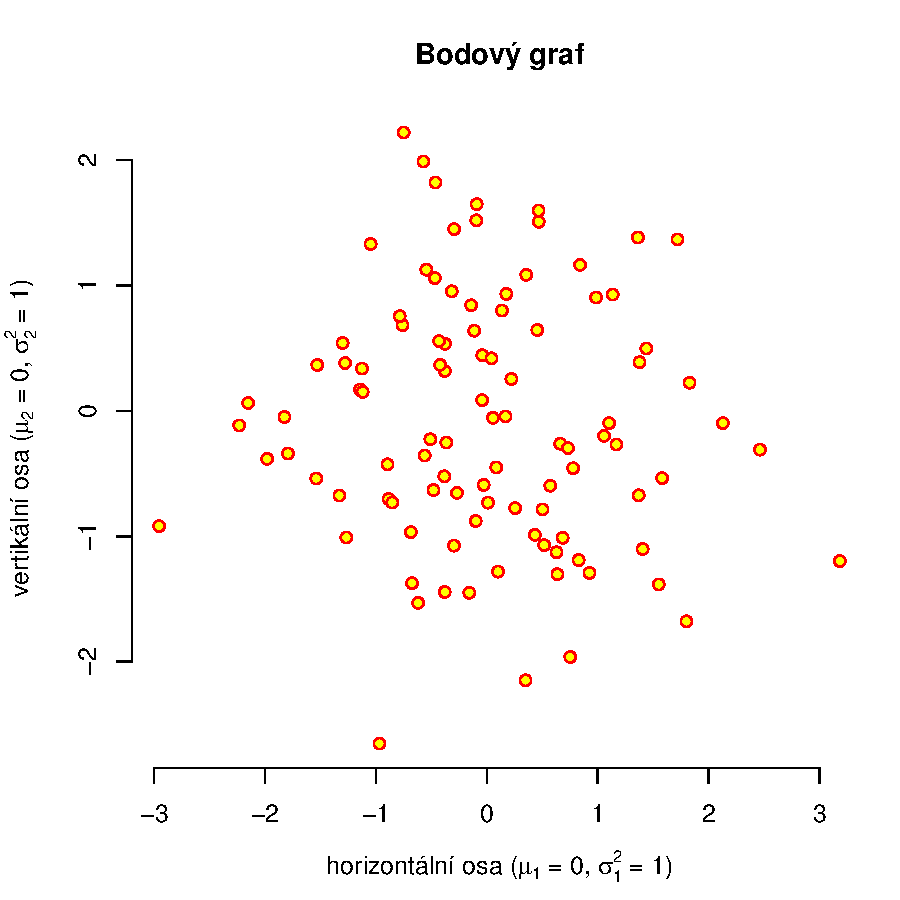
\includegraphics[width=.66\textwidth]{img/ukazka-obr01}
% Příponu není potřeba explicitně uvádět, pdflatex automaticky hledá pdf.
% Rozměry také není nutné uvádět.
\caption{Náhodný výběr z~rozdělení $\mathcal{N}_2(\boldsymbol{0},\,I)$.}
\label{obr03:Nvyber}
\end{figure}

Několik rad týkajících se obrázků a grafů.

\begin{itemize}
\item Graf by měl být vytvořen ve velikosti, v~níž bude použit
  v~práci. Zmenšení příliš velkého grafu vede ke špatné čitelnosti
  popisků.
\item Osy grafu musí být řádně popsány ve stejném jazyce, v~jakém je
  psána práce (absenci diakritiky lze tolerovat). Kreslíme-li graf
  hmotnosti proti výšce, nenecháme na nich popisky \texttt{ht} a
  \texttt{wt}, ale osy popíšeme \emph{Výška [cm]} a~\emph{Hmotnost
    [kg]}. Kreslíme-li graf funkce $h(x)$, popíšeme osy $x$ a $h(x)$.
  Každá osa musí mít jasně určenou škálu.
\item Chceme-li na dvourozměrném grafu vyznačit velké množství bodů,
  dáme pozor, aby se neslily do jednolité černé tmy. Je-li bodů mnoho,
  zmenšíme velikost symbolu, kterým je vykreslujeme, anebo vybereme
  jen malou část bodů, kterou do grafu zaneseme. Grafy, které obsahují
  tisíce bodů, dělají problémy hlavně v~elektronických dokumentech,
  protože výrazně zvětšují velikost souborů.
\item Budeme-li práci tisknout černobíle, vyhneme se používání barev.
  Čáry roz\-li\-šu\-je\-me typem (plná, tečkovaná, čerchovaná,\ldots), plochy
  dostatečně roz\-díl\-ný\-mi intensitami šedé nebo šrafováním. Význam
  jednotlivých typů čar a~ploch vysvětlíme buď v~textové legendě ke
  grafu anebo v~grafické legendě, která je přímo součástí obrázku.
\item Vyhýbejte se bitmapovým obrázkům o~nízkém rozlišení a zejména
  JPEGům (zuby a kompresní artefakty nevypadají na papíře pěkně).
  Lepší je vytvářet obrázky vektorově a vložit do textu jako PDF.
\end{itemize}


\section{Zdrojové kódy}
Algoritmy, výpisy programů a popis interakce s~programy je vhodné odlišit od ostatního textu. Jednou z~možností je použití {\LaTeX}o\-vé\-ho balíčku \texttt{listings}, pomocí něhož je v~souboru \texttt{makra.tex} nadefinováno jednoduché prostředí \texttt{code}. Pomocí něho lze vytvořit např. následující ukázky.

\begin{code}
> mean(x)
[1] 158.90
> objekt$prumer
[1] 158.90
\end{code}

Balíček \texttt{listings} a jeho prostředí \texttt{lstlisting} však nabízí téměř nepřeberné množství konfiguračních parametrů, např. pro zvýrazňování syntaxe programovacích jazyků (několika desítek), číslování řádku atd. Příklady:
\begin{itemize}
\item \url{https://en.wikibooks.org/wiki/LaTeX/Source_Code_Listings}
\item \url{https://www.overleaf.com/learn/latex/Code_listing#Using_listings_to_highlight_code}
\end{itemize}


\section{Sazba matematiky}
Proměnné sázíme kurzívou (to \TeX{} v~matematickém módu dělá sám, ale
nezapomínejte na to v~okolním textu a také si matematický mód zapněte).
Názvy funkcí sázíme vzpřímeně. Tedy například:
$\textrm{var} (X) = \textsf{E~} X^2 - \bigl(\textsf{E~} X \bigr)^2$.

Zlomky uvnitř odstavce (třeba $\frac{5}{7}$ nebo $\frac{x+y}{2}$) mohou
být příliš stísněné, takže je lepší sázet jednoduché zlomky s~lomítkem:
$5/7$, $(x+y)/2$.

Pro méně obeznámené se zvyklostmi v matematické sazbě lze doporučit stručný text od Richarda Starého -- \url{http://richardstary.wz.cz/clanky/matsaz/matsaz.pdf} --, který je obecně platný bez ohledu na to, zda použijete \LaTeX\ nebo Word.

Možnosti \LaTeX u pro sazbu matematiky jsou sice bohaté, ale je možné, že v některých specifických situacích nebudou postačovat. Proto lze doporučit k použití balíčky American Mathematical Society (AMS). V souboru \texttt{makra.tex} jsou standardně zaváděny balíčky \texttt{amsmath}, \texttt{amsfonts} a \texttt{amsthm}. Pro proniknutí do jejich možností poslouží:
\begin{itemize}
\item Math Extension with AMS\LaTeX\ -- \url{http://ptgmedia.pearsoncmg.com/images/0321173856/samplechapter/kopkach15.pdf}
\item \url{https://www.overleaf.com/learn/latex/Aligning_equations_with_amsmath}
\item Math Mode -- \url{http://tex.loria.fr/general/Voss-Mathmode.pdf}
\item More Math into LaTeX -- \url{http://tug.ctan.org/info/Math_into_LaTeX-4/Short_Course.pdf}
\end{itemize}

Ukázka číslovaného vzorce:
\begin{equation}
\mathbf{b}=(\mathbf{X}^\mathsf{T}\mathbf{X})^{-1}\mathbf{X}^\mathsf{T}\mathbf{y}
\end{equation}

Ukázka nečíslovaných vzorců s funkcemi a indexy:

$$
d_{ij}=\max_{k=1,2,\dots,n} \{d_{ik}+d_{kj}\},
$$
$$
x_{1,2}=b \pm \sqrt{\ln y}.
$$

Ukázku vzorce jako součást jednoho odstavce uveďme na příkladu kapacit dodavatelů v matematickém modelu dopravního problému, které zohledníme pomocí omezení:
\begin{equation}
\sum_{j=1}^n x_{ij} \le a_i, \qquad i=1,2,\dots,m\ ,
\end{equation}
\noindent
kde výraz $a_i$ představuje kapacitu $i$-tého dodavatele.

Při odvozování vzorce postupnou úpravou se obvykle jednotlivé kroky uvádějí na samostatných řádcích (prostředí \verb'align*' z balíčku \verb|amsmath|):
\begin{align*}
 f(x) &= (x+a)(x+b) =\\
      &= x^2 + bx + ax + ab =\\
      &= x^2 + (a+b)x + ab
\end{align*}

Ukázka sloupcové úpravy (\verb|eqnarray*|):
\begin{eqnarray*}
\sum_{i=1}^n x_{ij} =1, && j=1,2,\dots,n,\\
\sum_{j=1}^n x_{ij} =1, && i=1,2,\dots,n,\\
u_i + 1 - M(1 - x_{ij}) \le u_j, && i=2,3,\dots,n,\quad j=1,2,\dots,n,\\
u_i \ge 0,              && i=1,2,\dots,n,\\
x_{ij} \in \{0,1\} && i=1,2,\dots,n,\quad j=1,2,\dots,n,\\
\end{eqnarray*}
%%% Fiktivní kapitola s ukázkami citací

\chapter{Práce s literaturu}

Šablona předpokládá použití bibliografické databáze z důvodu větší flexibility. Použití bibliografické databáze není nutnou podmínkou, lze si vystačit i se standardním prostředím \texttt{thebibliography}. V takovém případě je však zapotřebí provést zásahy do některých souborů, jak je uvedeno dále.

\section{Použití bibliografické databáze}

\begin{enumerate}
\item\textbf{Změna názvu databáze}\\
V šabloně se předpokládá databáze uložená v souboru \texttt{literatura.bib}. Pokud se databáze jmenuje jinak, pak je nutné v souboru \texttt{makra.tex} změnit hodnotu parametru příkazu \verb'\bibliography'.
\item\textbf{Změna citačního stylu}\\
Standardně se citace v textu uvádějí v číselné variantě. Na použití kombinace příjmení a roku lze snadno přepnout změnou v souboru \texttt{makra.tex}, kde se prohodí komentářový znak v parametrech pro balíček \texttt{biblatex}.
\end{enumerate}


\section{Použití prostředí \texttt{thebibliography}}
\begin{enumerate}
\item V souboru \texttt{makra.tex} vymazat na počátku tyto řádky:
\begin{verbatim}
%%% Nastavení pro použití samostatné bibliografické databáze.
%%% Settings for using a separate bibliographic database.
\usepackage[
   backend=biber
%  ,style=iso-authoryear
  ,style=iso-numeric
  ,sortlocale=cs_CZ
  ,alldates=iso
  ,bibencoding=UTF8
  ,maxnames=2
  ,maxbibnames=99
  %,block=ragged
]{biblatex}
\let\cite\parencite
\renewcommand*{\multinamedelim}{, \addspace}
\renewcommand*{\finalnamedelim}{\addspace a \addspace}

\bibliography{literatura}
\end{verbatim}
\item V souboru \texttt{literatura.tex} odstranit řádek s příkazem \verb'\printbibliography' a odstranit příznak komentáře v další části obsahující prostředí \texttt{thebibliography.}
\end{enumerate}


\section{Jak citovat v textu}
\begin{center}
\begin{tabular}{l@{~~$\longrightarrow$~~}l}
\verb|\cite{Cermak2018}|&\cite{Cermak2018}\\
\verb|\cite{Hladik2018,Jasek2018}|&\cite{Hladik2018,Jasek2018}\\
\verb|\cite[kap. 3]{Pecakova2018}|&\cite[kap. 3]{Pecakova2018}\\
\end{tabular}
\end{center}

%%% Fiktivní kapitola s instrukcemi k PDF/A

\chapter{Formát PDF/A}

Elektronická podoba závěrečných
prací musí být odevzdávána ve formátu PDF/A úrovně 1a nebo 2u. To jsou
profily formátu PDF určující, jaké vlastnosti PDF je povoleno používat,
aby byly dokumenty vhodné k~dlouhodobé archivaci a dalšímu automatickému
zpracování. Dále se budeme zabývat úrovní 2u, kterou sázíme \TeX{}em.

Mezi nejdůležitější požadavky PDF/A-2u patří:

\begin{itemize}

\item Všechny fonty musí být zabudovány uvnitř dokumentu. Nejsou přípustné
odkazy na externí fonty (ani na \uv{systémové}, jako je Helvetica nebo Times).

\item Fonty musí obsahovat tabulku ToUnicode, která definuje převod z~kódování
znaků použitého uvnitř fontu to Unicode. Díky tomu je možné z~dokumentu
spolehlivě extrahovat text.

\item Dokument musí obsahovat metadata ve formátu XMP a je-li barevný,
pak také formální specifikaci barevného prostoru.

\end{itemize}

Tato šablona používá balíček {\tt pdfx,} který umí \LaTeX{} nastavit tak,
aby požadavky PDF/A splňoval. Metadata v~XMP se generují automaticky podle
informací v~souboru {\tt prace.xmpdata} (na vygenerovaný soubor se můžete
podívat v~{\tt pdfa.xmpi}).

Správnost PDF/A lze zkontrolovat pomocí on-line validátoru: \url{https://www.pdf-online.com/osa/validate.aspx/}.

Pokud soubor nebude validní, mezi obvyklé příčiny patří používání méně
obvyklých fontů (které se vkládají pouze v~bitmapové podobě a/nebo bez
unicodových tabulek) a vkládání obrázků v~PDF, které samy o~sobě standard
PDF/A nesplňují.

Je pravděpodobné, že se to týká obrázků vytvářených mnoha různými programy.
V~takovém případě se můžete pokusit obrázek do zkonvertovat do PDF/A pomocí
GhostScriptu, například takto:

\begin{verbatim}
        gs -q -dNOPAUSE -dBATCH
           -sDEVICE=pdfwrite -dPDFSETTINGS=/prepress
           -sOutputFile=vystup.pdf vstup.pdf
\end{verbatim}

% \include{...}
% \include{...}
{%
\pagestyle{plain}
\chapter*{Závěr}
\addcontentsline{toc}{chapter}{Závěr}

Závěr je povinnou částí bakalářské/diplomové práce. Obsahuje shrnutí práce a vyjadřuje se k míře splnění cíle, který byl v práci stanoven, případně shrnuje odpovědi na otázky, které byly položeny v úvodu práce. 

Závěr k diplomové práci musí být propracovanější -- podrobněji to je uvedeno v Náležitostech diplomové práce v rámci Intranetu pro studenty FIS.

Závěr je vnímán jako kapitola (chapter), která začíná na samostatné stránce a která má název Závěr.  Název Závěr se nečísluje. Samotný text závěru je členěn do odstavců.
}

%%% Seznam použité literatury
%%% Bibliography
%% Toto platí v případě použití samostatné bibliografické databáze
\printbibliography[title={\bibname},heading={bibintoc}]

%% Toto platí v případě použití prostředí thebibliography
%% Pro sestavení citačních údajů lze doporučit:
%%     https://knihovna.vse.cz/citace/priklady/
%%     https://www.citace.com/
%\openright
%\phantomsection
%\addcontentsline{toc}{chapter}{\bibname}
%\begin{thebibliography}{99}
%\bibitem{Cermak2018}ČERMÁK, Radim, SMUTNÝ, Zdeněk. A Framework for Cultural Localization of Websites and for Improving Their Commercial Utilization. In:  \emph{Global Observations of the Influence of Culture on Consumer Buying Behavior} [online]. Hershey~: IGI Global, 2018, s. 206--232. ISBN 978-1-5225-2727-5. DOI: 10.4018/978-1-5225-2727-5.
%
%\bibitem{Hladik2018}HLADÍK, Milan, ČERNÝ, Michal. The Shape of the Optimal Value of a Fuzzy Linear Programming Problem. In: \emph{Fuzzy Logic in Intelligent System Design} [online]. Cancum, 16.10.2017 -- 18.10.2017. Cham~: Springer, 2018, s. 281--286. Advances in Intelligent Systems and Computing 648. ISBN 978-3-319-67136-9. DOI: 10.1007/978-3-319-67137-6\_31.
%
%\bibitem{Jasek2018}JAŠEK, Pavel, VRANÁ, Lenka, ŠPERKOVÁ, Lucie, SMUTNÝ, Zdeněk, KOBULSKÝ, Marek. Modeling and Application of Customer Lifetime Value in Online Retail. \emph{Informatics} [online]. 2018, roč. 5, č. 1. 22 s. eISSN 2227-9709. DOI: 10.3390/informatics5010002. Dostupné také z: \url{http://www.mdpi.com/2227-9709/5/1/2/pdf}.
%
%\bibitem{Pecakova2018}PECÁKOVÁ, Iva. \emph{Statistika v terénních průzkumech}. 3. přeprac. vyd. Praha~: Professional Publishing, 2018. 254 s. ISBN 978-80-88260-10-3.
%\end{thebibliography}


%%% Přílohy k práci, existují-li. Každá příloha musí být alespoň jednou
%%% odkazována z vlastního textu práce. Přílohy se číslují.
%%% Attachments to thesis, if any. Each attachment must be referenced at 
%%% least once in your own text. The appendices are numbered.
\part*{\Prilohy\thispagestyle{empty}}
\appendix
\chapter{Formulář v plném znění}


\chapter{Zdrojové kódy výpočetních procedur}


% \include{...}
% \include{...}

\end{document}
